
This chapter provides important artifacts related to design of our project.

% Your report will contain ONE of the following 2 sections.

\section{Data Design}

This section presents the structure of our database that caters to persistent data storage in our project. The structure is shown as a normalized data model for relational databases. It clearly shows entities, attributes, relationships with their cardinalities, and primary and foreign keys. We have used DB designer to build our data model.


\begin{figure}[H]
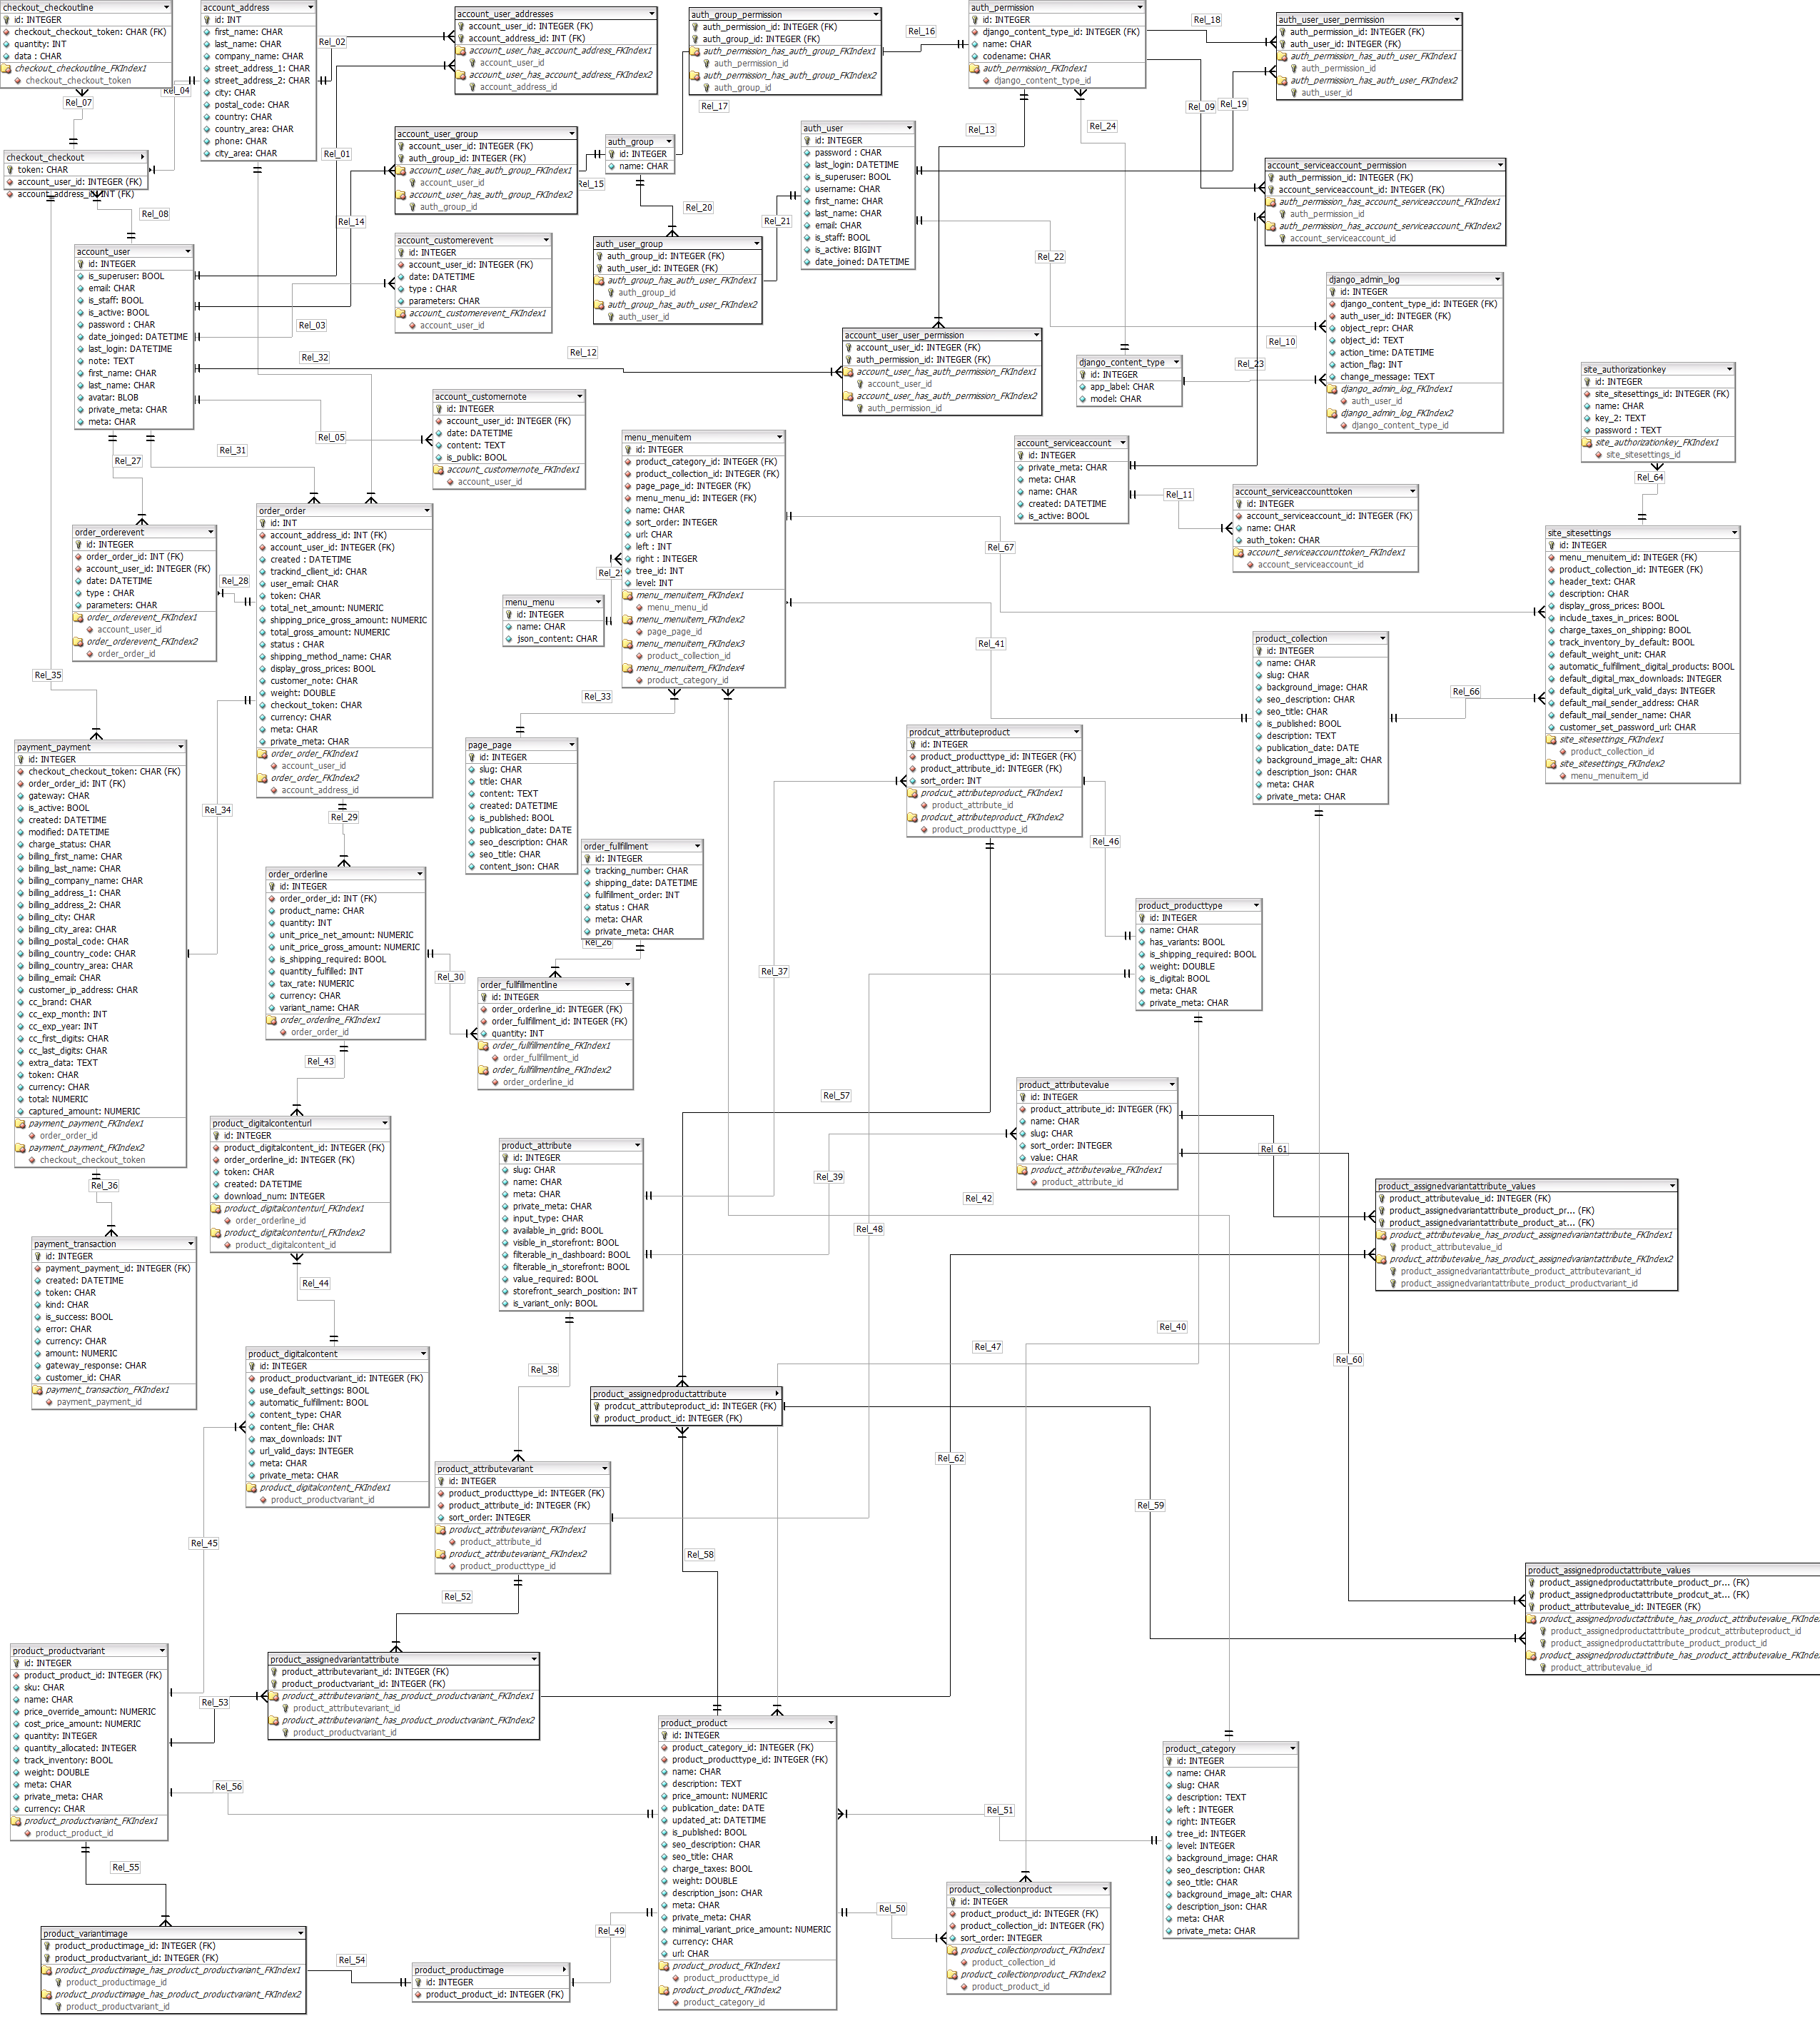
\includegraphics[width=15cm, height = 18cm, keepaspectratio]{images/PORS_ERD.png} 
\centering
\caption{Entity Relationship Diagram}
\label{erd}
\end{figure}
 
%\section{Technical Details}
%
%Our project does not have persistent data so we have no ERD. Instead we exaplin here the technical details of the algortihsm we use. These include the inputs and the outputs, how and where these algorothms fit in our tool chain, the techniques used in these algorithms, etc.

\section{State Diagram}

\begin{figure}[H]
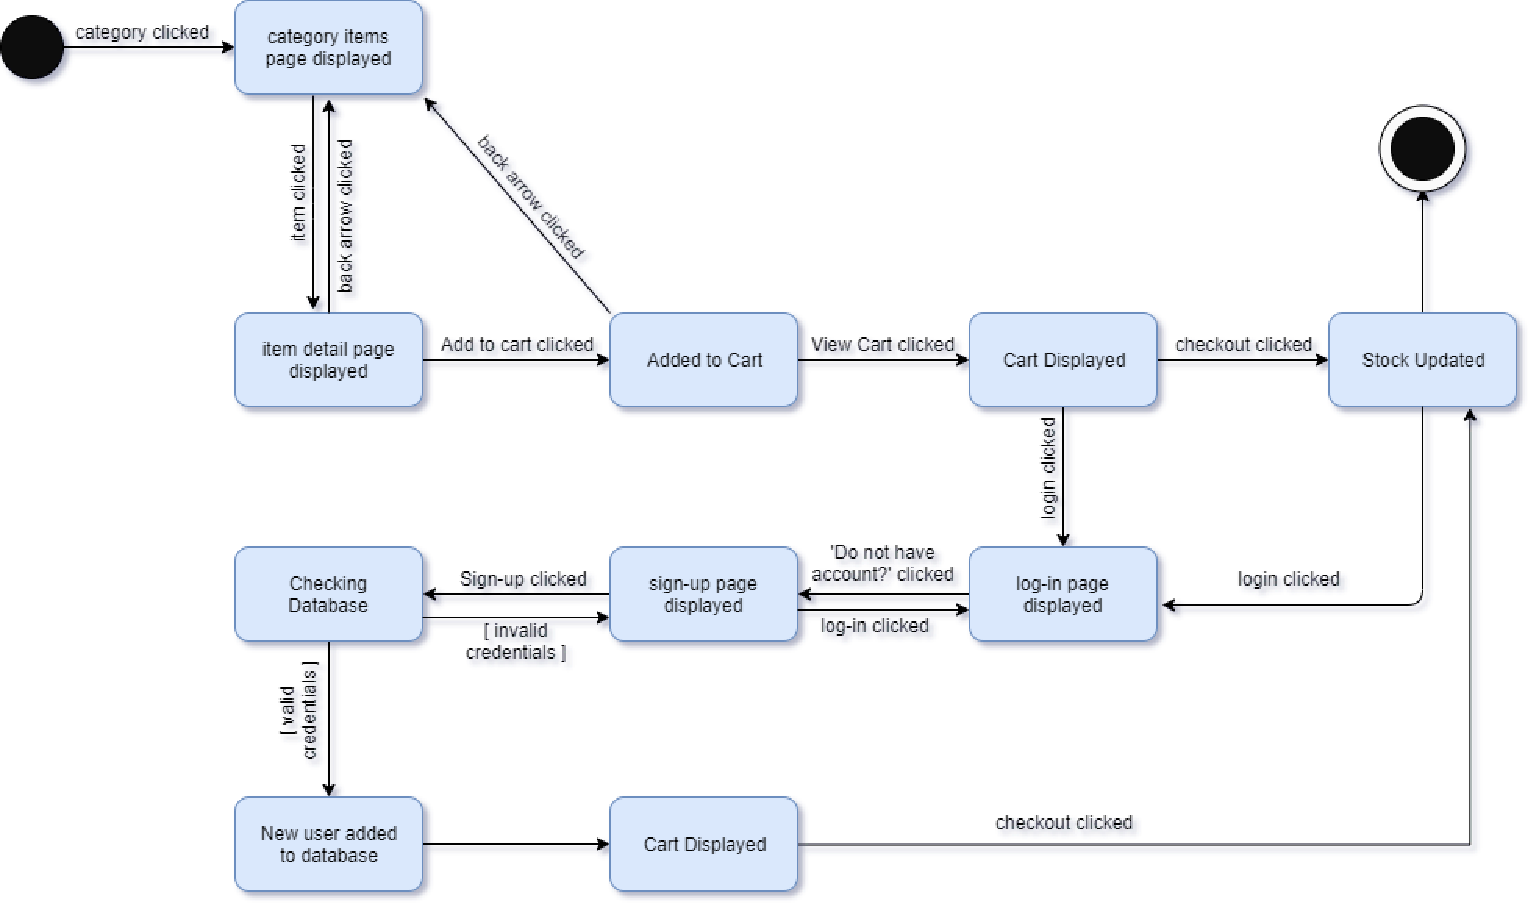
\includegraphics[width=10cm]{images/StateDiag1.pdf} 
\centering
\caption{State Diagram 1}
\label{state: one}
\end{figure}

\begin{figure}[H]
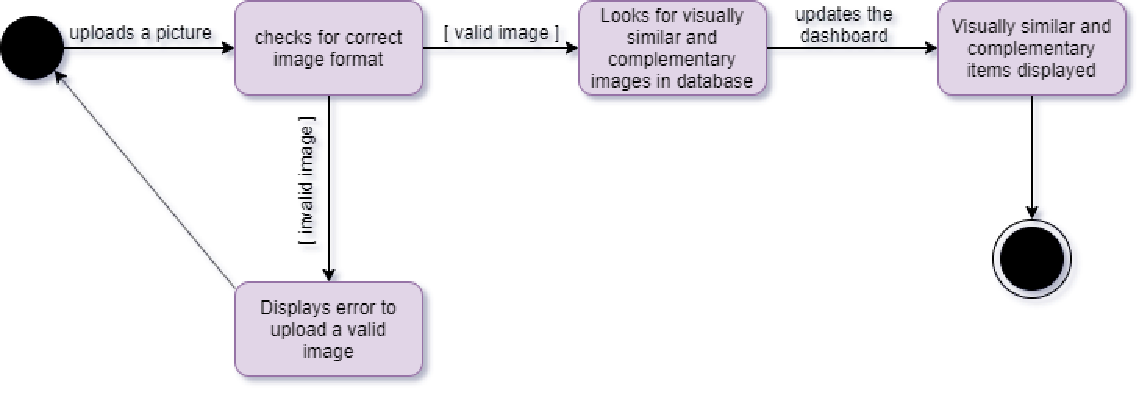
\includegraphics[width=10cm]{images/StateDiag2.pdf} 
\centering
\caption{State Diagram 2}
\label{state: two}
\end{figure}

\section{Sequence Diagram}
\begin{figure}[H]
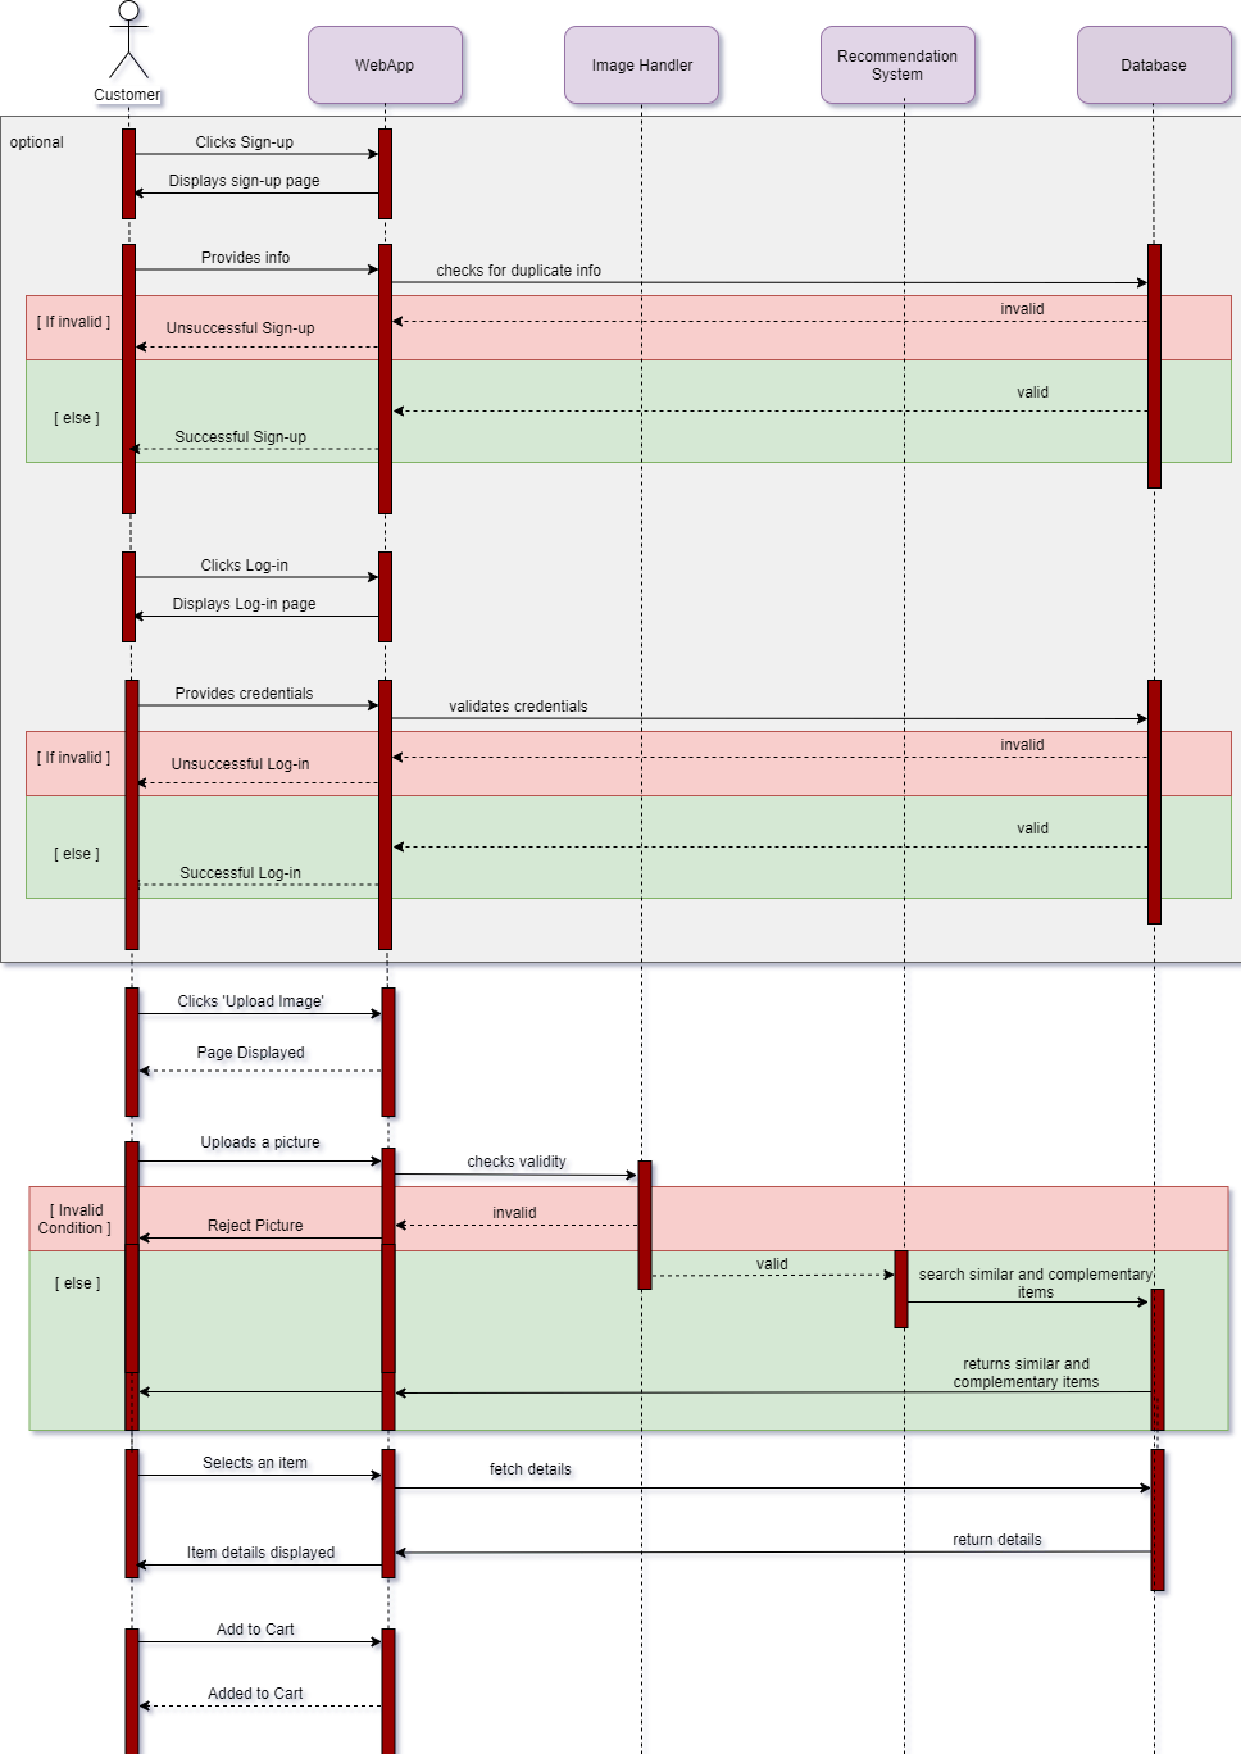
\includegraphics[width=12cm]{images/SequenceDiag1.pdf} 
\centering
\caption{Sequence Diagram - Customer}
\label{sequence: one}
\end{figure}